\todo{Do it.}

\section{Client Participation}

\begin{figure}[!ht]
    \centering
    \centering
    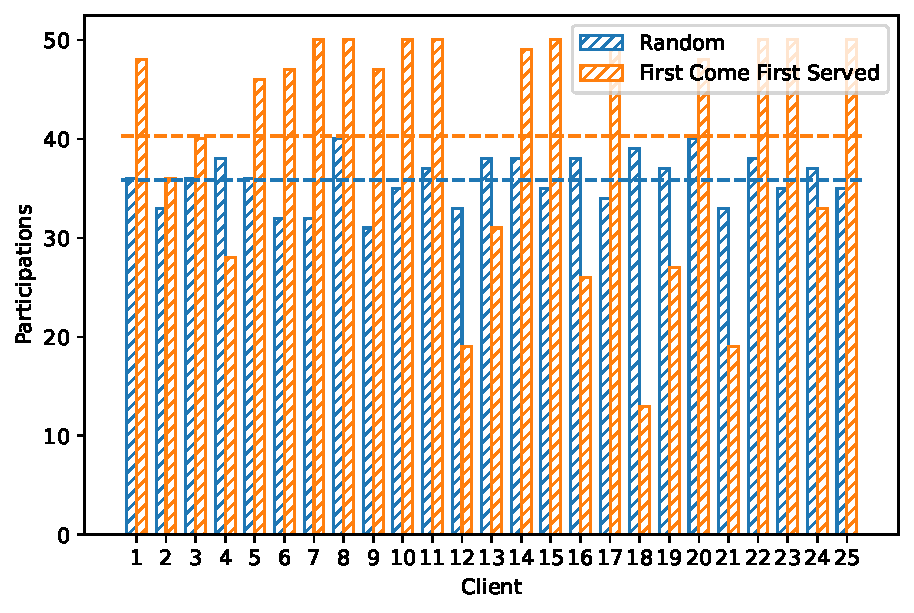
\includegraphics[width=0.7\textwidth]{graphics/selection/clients.pdf}
    \caption{Participation of Each Client Per Selection Technique}
    \label{fig:participations_client}
\end{figure}

\section{Execution Time, Transaction Cost and Latency}

\begin{table}[!ht]
\begin{tabular}{c|c|c} \hline \hline
                              & First Come First Served & Random \\ \hline \hline
E2E Time (m)                   & 19.70                   & 18.93  \\ \hline
Mean Round Time (s)            & 23.62                   & 22.70  \\ \hline
% Median Round Time (s)          & 22.06                   & 21.90  \\ \hline
Mean Transaction Latency (s)   & 1.560                   & 1.549  \\ \hline
% Median Transaction Latency (s) & 1.561                   & 1.549  \\ \hline
Mean Transaction Cost (Gas)    & 189179                  & 183124 \\ \hline
% Median Transaction Cost (Gas)  & 223471                  & 185198 \\ \hline
\end{tabular}
\caption{Time and Transaction Metrics Per Participant Selection Technique}
\label{tab:metrics_selection}
\end{table}

\section{Accuracy and Convergence}

\begin{figure}[!ht]
    \centering
    \centering
    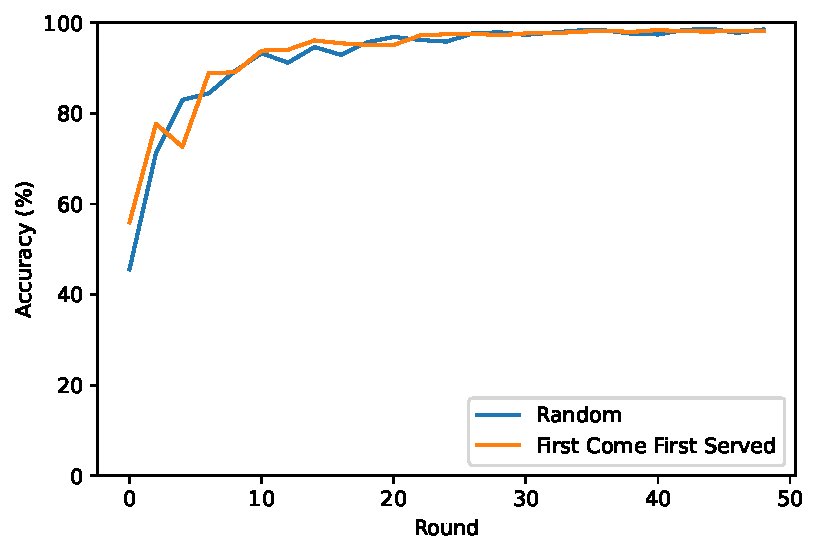
\includegraphics[width=0.7\textwidth]{graphics/selection/accuracy.pdf}
    \caption{Accuracy Per Participant Selection Technique}
    \label{fig:accuracy_selection}
\end{figure}

\section{Communication Costs}

\begin{figure}[!ht]
    \centering
    \centering
    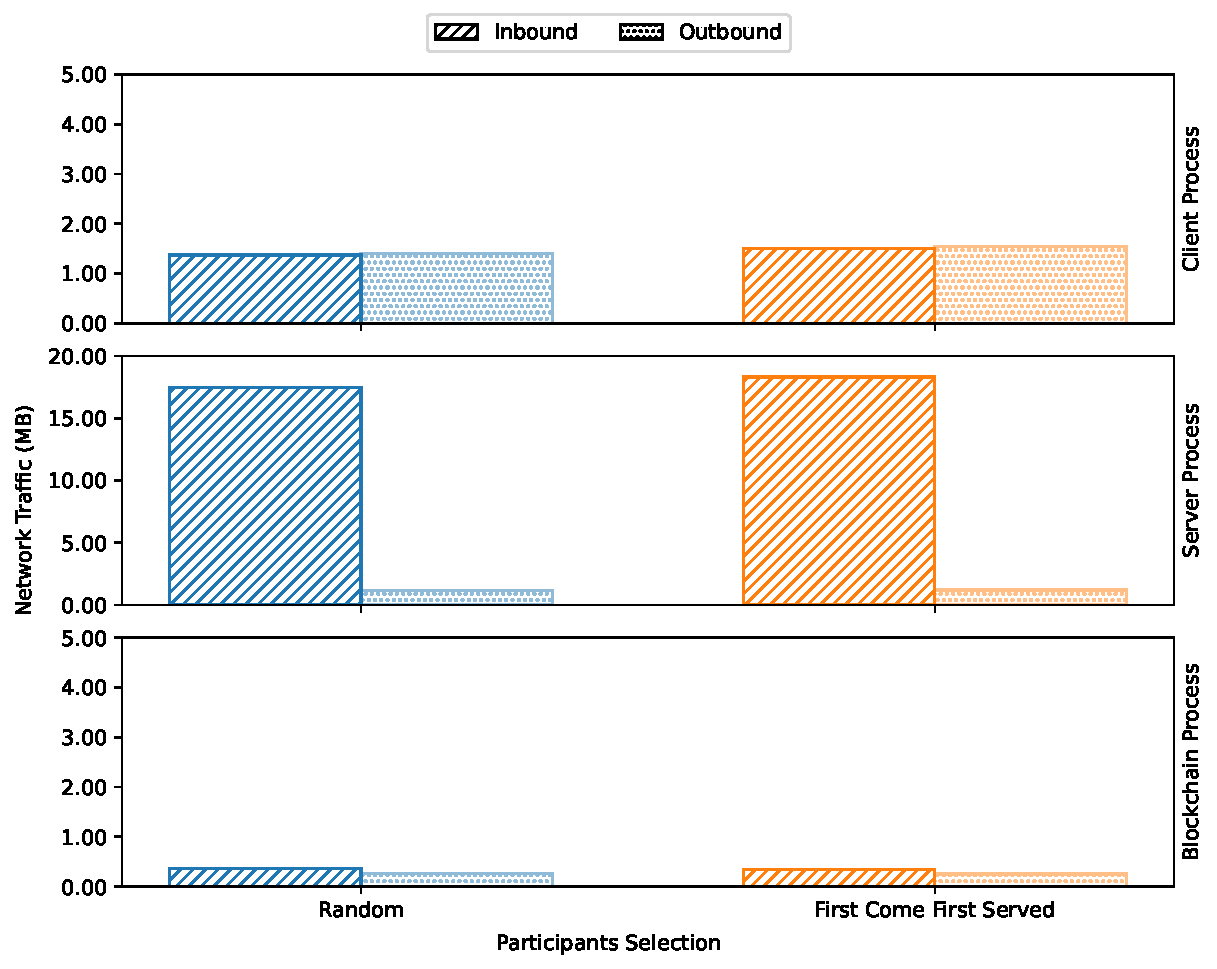
\includegraphics[width=0.8\textwidth]{graphics/selection/net.pdf}
    \caption{Network Traffic Per Round Per Participant Selection Technique}
    \label{fig:net_selection}
\end{figure}

\section{Computation Costs}

\begin{figure}[!hpt]
    \centering
    \centering
    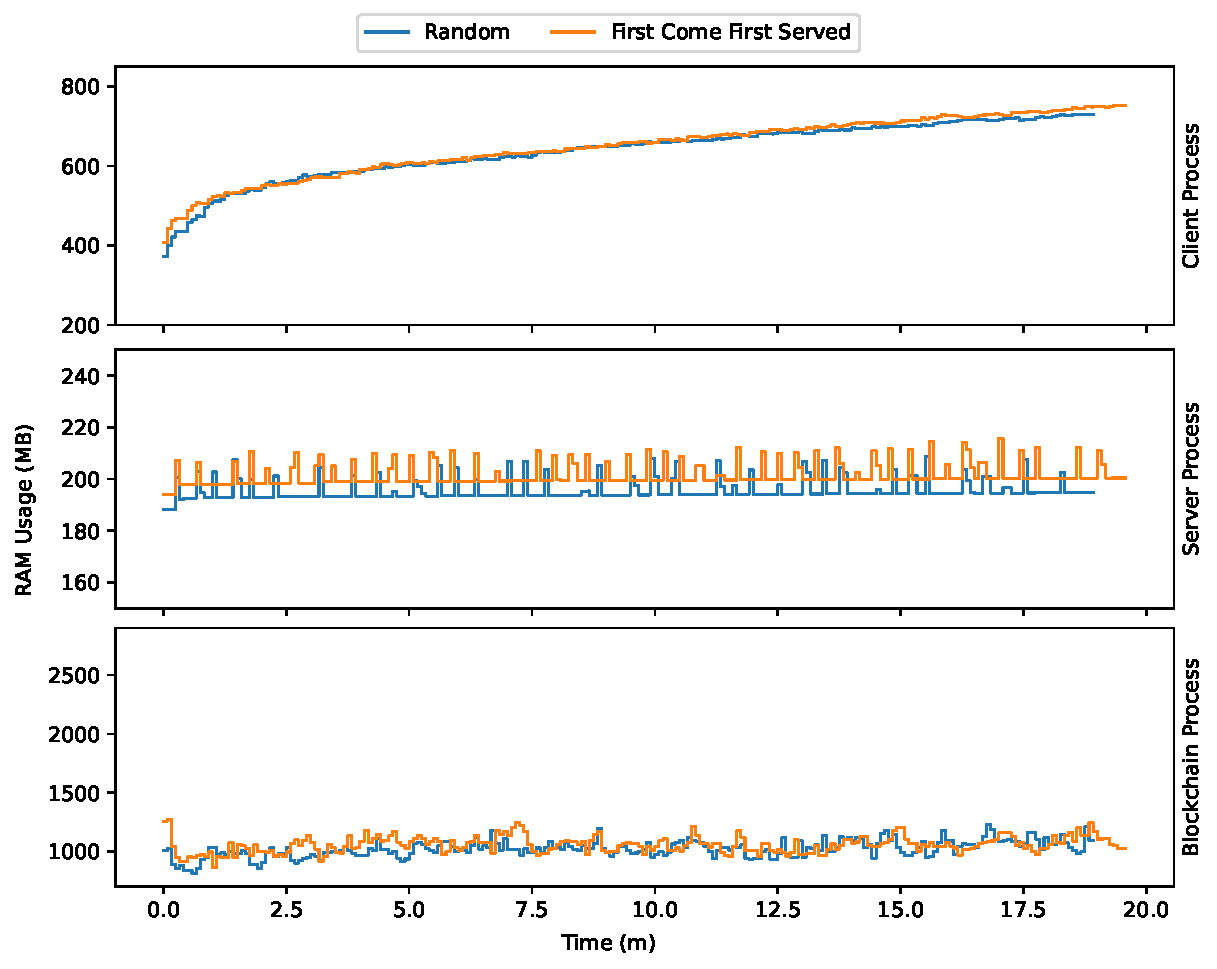
\includegraphics[width=0.8\textwidth]{graphics/selection/ram.pdf}
    \caption{RAM Usage Per Participant Selection Technique}
    \label{fig:ram_selection}
\end{figure}

\begin{figure}[!hpb]
    \centering
    \centering
    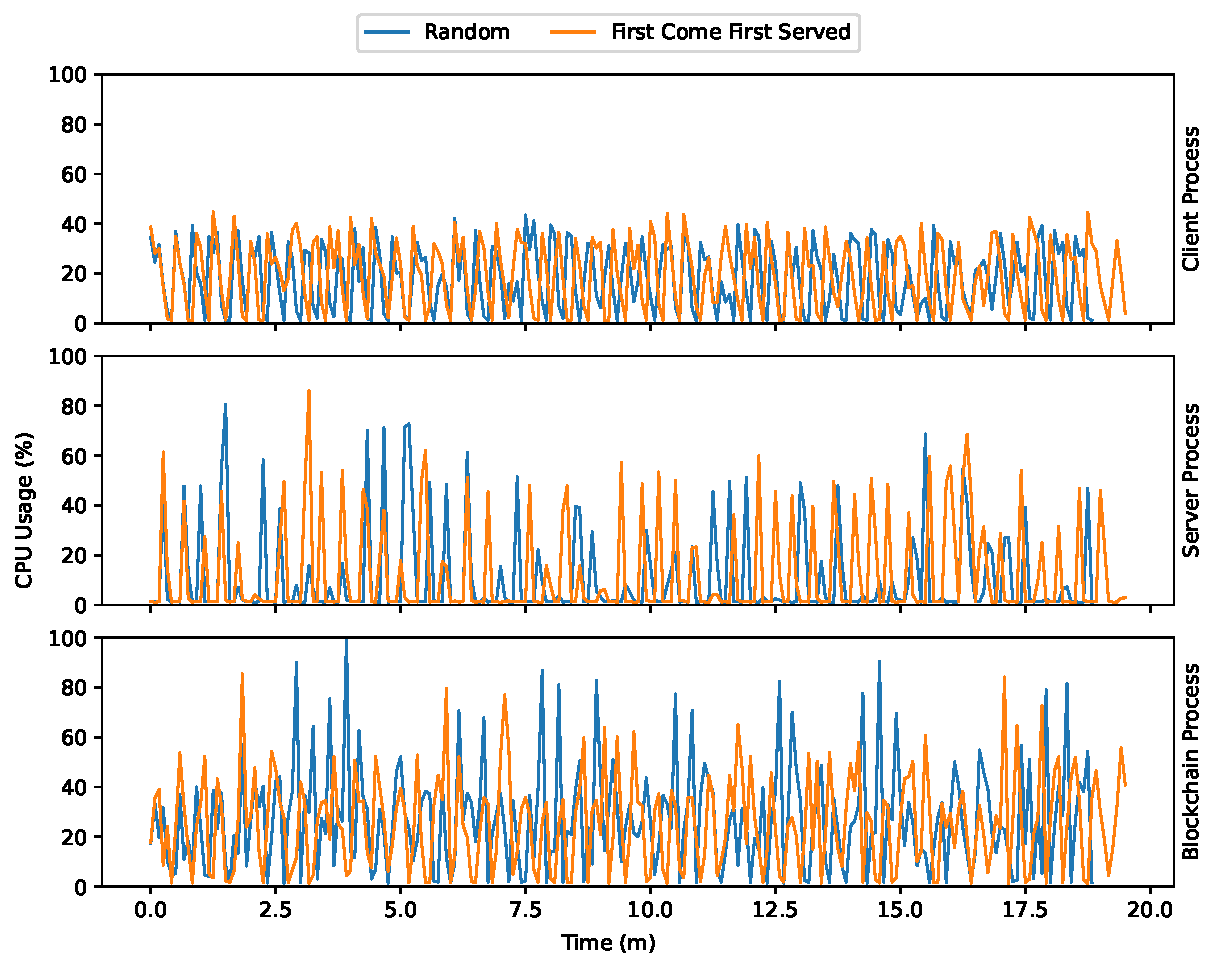
\includegraphics[width=0.8\textwidth]{graphics/selection/cpu.pdf}
    \caption{CPU Usage Per Participant Selection Technique}
    \label{fig:cpu_selection}
\end{figure}

\section{Conclusions} % and improvements? and limitations?
